\section{Experiments} \label{sec:exp}
%\vspace{-0.25cm}

A prototype\footnote{Source code available at \url{https://github.com/jgorzny/Skeptik}} version of {\FORPI} has been implemented in the functional programming language Scala as part of the \skeptik
library. This library includes an implementation of {\GFOLU} \cite{GFOLU}. In order to evaluate the algorithm's effectiveness, {\FORPI} was tested on two data sets: proofs generated by a real theorem prover and artificial proofs resolution proofs. The data is included in the source code repository.

First, {\FORPI} was evaluated on the same set of proofs used to evaluate {\GFOLU}. This data was generated by executing the {\SPASS} ({\url{http://www.spass-prover.org/}) theorem prover on 2280 real first-order problems without equality of the TPTP Problem Library (among them, 1032 problems are known to be unsatisfiable). In order to generate pure resolution proofs, the advanced inference rules of {\SPASS} were disabled. The proofs were originally generated on the Euler Cluster at the University of Victoria with a time limit of 300 seconds per problem. Under these conditions, {\SPASS} generated 308 proofs. The proofs generated by SPASS were small: proof lengths varied from 3 to 49, and the number of resolutions in a proof ranged from 1 to 32.

In order to test {\FORPI}'s effectiveness on larger proofs, randomly generated first-order resolution proofs were also used.
Proofs were generated by 
In order to match the maximum number of potential proofs from the TPTP Problem Library, 2280 randomly generated proofs were used as the second data set. The proofs generated by were much larger than those of the first data set: proof lengths varied from 95 to 700, while the number of resolutions in a proof ranged from 48 to 368.

In order to maintain consistency, the same system and metrics were used. Proof compression and proof generation was performed on a laptop (2.8GHz Intel Core i7 processor with 4GB of RAM (1333MHz DDR3) available to the Java Virtual Machine); proofs from the first data set were not generated again. For each proof $\psi$, we measured the time needed to compress the proof ($t(\psi)$) and the compression ratio in terms of resolutions ($(|\psi|-|\alpha(\psi)|)/|\psi|$) where $|\psi|$ is the number of resolutions in the proof, and $\alpha(\psi)$ is the result of applying a compression algorithm or the composition of {\FORPI} and {\GFOLU}.

Only nine proofs from the TPTP data set were compressed by {\FORPI}, reducing the number of resolutions by at least one but at most three. However, 252 (0.11\%) of the randomly generated proofs achieved some compression using only {\FORPI}.
Figure \ref{fig:forpimean} shows a box-whisker plot of compression ratio with proofs grouped by number of resolutions and whiskers indicating a minimum and maximum compression ratio achieved within the group. The circles indicate the mean compression ratio when considering only proofs for which some compression was achieve, and these points indicate that when larger proofs can be compressed, they are compressed more than smaller proofs.
{\FORPI} was able to achieve an overall average compression ratio 5\% on this data. The compression ratio for only the compressed proofs is 33\%, compared to 13\% for {\GFOLU}.

Figure \ref{fig:ex} (a) shows the number of proofs (compressed and uncompressed) per grouping based on number of resolutions in the proof. The red (respectively dark gray) data shows the number of compressed (respectively, uncompressed) proofs for the TPTP data set, while the green (respectively light gray) data shows the number of compressed (respectively, uncompressed) proofs for the random proofs. Darker colours indicate the number of proofs compressed by both {\FORPI} and {\GFOLU} and both compositions of these algorithms; lighter colours indicate cases were {\FORPI} succeeded, but at least one of {\GFOLU} or a combination of these algorithms achieved no compression. The random proofs indicate that many proofs have some irregularity, but this is not reflected in the TPTP data; this is unsurprising given the size of the proofs in the TPTP data set.

Figure \ref{fig:ex} (b) shows a scatter plot comparing the number resolutions of the input proof against the number of resolutions in the compressed proof. The data resulting from the TPTP data is magnified by the internal plot. For the randomly generated proofs (points to the left of the blown-up area), it is often the case that the length of the compressed proof is significantly lesser than the length of the input proof. In some cases, {\FORPI} is able to reduce the number of resolutions from the hundreds to single digit values. Interestingly, {\GFOLU} appears to reduce the the number of resolutions by a linear factor. We conjecture that this is due to the method by which the data was generated: specifically, ... TODO

Figure \ref{fig:ex} (c) shows a scatter plot comparing the size of compression obtained by applying {\FORPI} before {\GFOLU} versus {\GFOLU} before {\FORPI}. Data generated from the TPTP data set is marked in red; the rest are obtained from random proofs. Points that lie on the line $y=x$ have the same size after both combinations. 165 points lie beneath the line, while 258 are above the line. This suggests that {\GFOLU} should be applied after {\FORPI}: to maximize the likelihood of compression, in addition to maximizing the compression.

Figure \ref{fig:ex} (d) shows a plot comparing the difference in the cumulative number resolutions of the first $x$ input proofs against the cumulative number of resolutions in the first $x$ compressed proofs. Again, the TPTP data is magnified in the sub-plot. Where, we see that the use of both algorithms is always better than using a single algorithm, and further that applying {\FORPI} after {\GFOLU} appears to be the best option.



{\SPASS} required approximately 40 minutes (running on a cluster and including proof generation time for each problem) to solve the generated proofs. The total time for {\GFOLU} and {\FORPI} to be executed on all 308 TPTP proofs was just under X seconds on a simple laptop. The random proofs were generated in X seconds, and took approximately X minutes to compress, both measured on a laptop.
All times including parsing time. These compression algorithms continue to be very fast, and may simplify the proof considerably for a relatively quick time cost.

%the compression obtained by applying {\FORPI} and {\GFOLU} (as well as their combinations) to the proofs. 
%Unsurprisingly, applying both algorithms generally does better than either algorithm alone. 
%With this data set, {\FORPI} compresses a few proofs only, and its performance is not as good as that of {\GFOLU}. Furthermore, when {\FORPI} is combined with {\GFOLU}, {\FORPI} provides additional compression to only three proofs already compressed by {\GFOLU}. This is surprising, because in the propositional case, {\RPI} usually compresses up to ten times more than {\LowerUnits}. Nevertheless, this can be easily explained by the fact that all available benchmark proofs have small heights (not more than 11); consequently the path from any node to the root is short and unlikely to contain irregularities. In the propositional case, on the other hand, {\RPI} has been tested on proofs that are a thousand times higher.





% although more data is needed for confirmation. The number of points above and below the main diagonal are the same; however, the points below may simply be the result of {\GFOLU} being more likely to compress such short proofs. If so, that would imply that running {\FORPI} after {\GFOLU} is more successful, which would be consistent with propositional results for these algorithms.
%Running {\FORPI} after {\GFOLU} shows some compression that...
%This is consistent with propositional results for these algorithms.

%Before evaluating this algorithm, we first generated several benchmark proofs. This was done by executing the {\SPASS}\footnote{\url{http://www.spass-prover.org/}} theorem prover on 2280 real first-order problems without equality of the TPTP Problem Library \footnote{\url{http://www.cs.miami.edu/{\textasciitilde}tptp/}} (among them, 1032 problems are known to be unsatisfiable). In order to generate pure resolution proofs, most advanced inference rules used by {\SPASS}  were disabled. The Euler Cluster at the University of Victoria\footnote{\url{https://rcf.uvic.ca/euler.php}} was used and the time limit was 300 seconds per problem. Under these conditions, {\SPASS} was able to generate 308 proofs. 


%The proofs generated by {\SPASS} were small (with lengths from 3 to 49). These proofs are specially small in comparison with the typical proofs generated by SAT- and SMT-solvers, which usually have from a few hundred to a few million nodes. The number of proofs (compressed and uncompressed) per length is shown in Figure \ref{fig:ex} (b). Uncompressed proofs are those which had either no lowerable units to lower or for which \SFOLowerUnits failed and returned the original proof. Such failures occurred on only 14 benchmark proofs. Among the smallest of the 308 proofs, very few proofs were compressed. This is to be expected, since the likelihood that a very short proof contain a lowerable unit (or even merely a unit with more than one child) is low. The proportion of compressed proofs among longer proofs is, as expected, larger, since they have more nodes and it is more likely that some of these nodes are lowerable units. 13 out of 18 proofs with length greater than or equal to 30 were compressed. 

%Figure \ref{fig:ex} (a) shows a box-whisker plot of compression ratio with proofs grouped by length and whiskers indicating minimum and maximum compression ratio achieved within the group. Besides the median compression ratio (the horizontal thick black line), the chart also shows the mean compression ratios for all proofs of that length and for all compressed proofs (the red cross and the blue circle). In the longer proofs (length greater than 34), the median and the means are in the range from 5\% to 15\%, which is satisfactory in comparison with the total compression ratio of 7.5\% that has been measured for the propositional {\LowerUnits} algorithm on much longer propositional proofs \cite{Boudou}.

%Figure \ref{fig:ex} (c) shows a scatter plot comparing the length of the input proof against the length of the compressed proof. For the longer proofs (circles in the right half of the plot), it is often the case that the length of the compressed proof is significantly lesser than the length of the input proof.

%Figure \ref{fig:ex} (d) plots the cumulative original and compressed lengths of all benchmark proofs (for an x-axis value of $k$, the cumulative curves show the sum of the lengths of the shortest $k$ input proofs). The total cumulative length of all original proofs is 4429 while the cumulative length of all proofs after compression is 3929. This results in a total compression ratio of 11.3\%, which is impressive, considering that the inclusion of all the short proofs (in which the presence of lowerable units is a priori unlikely) tends to decrease the total compression ratio. For comparison, the total compression ratio considering only the 100 longest input proofs is 18.4\%.

%Figure \ref{fig:ex} also indicates an interesting potential trend. The gap between the two cumulative curves seems to grow superlinearly. If this trend is extrapolated, progressively larger compression ratios can be expected for longer proofs. This is compatible with Theorem 10 in \cite{LURPI}, which shows that, for proofs generated by eagerly resolving units against all clauses, the propositional {\LowerUnits} algorithm can achieve quadratic assymptotic compression. SAT- and SMT-solvers based on CDCL (Conflict-Driven Clause Learning) avoid eagerly resolving unit clauses by dealing with unit clauses via boolean propagation on a conflict graph and extracting subproofs from the conflict graph with every unit being used at most once per subproof (even when it was used multiple times in the conflict graph). Saturation-based automated theorem provers, on the other hand, might be susceptible to the eager unit resolution redundancy described in Theorem 10 \cite{LURPI}. This potential trend would need to be confirmed by further experiments with more data (more proofs and longer proofs).


%TODO: change time
%{\SPASS} required approximately 40 minutes to solve and generate the proofs; the total time for {\GFOLU} and {\FORPI} to be executed on all 308 proofs was just under 8 seconds (both include parsing time).

\begin{figure}[bt]
\centering
  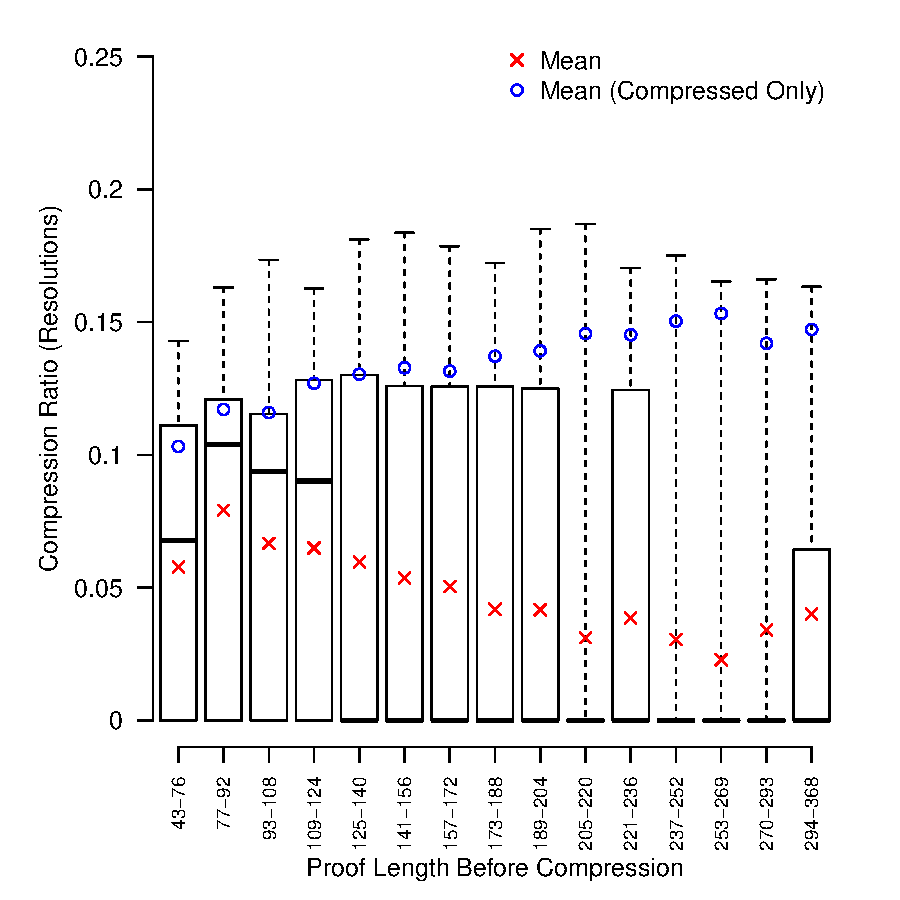
\includegraphics[scale=0.5]{images/final-random-forpi-compress_ratio_res_vs_proof_res_length.pdf}
  
    \caption{Compression Ratio (\FORPI)}
    \label{fig:forpimean}
    \end{figure}

\begin{figure}[p]
    
    \hspace{-2cm}\subfloat[Number of (non-)compressed proofs]{{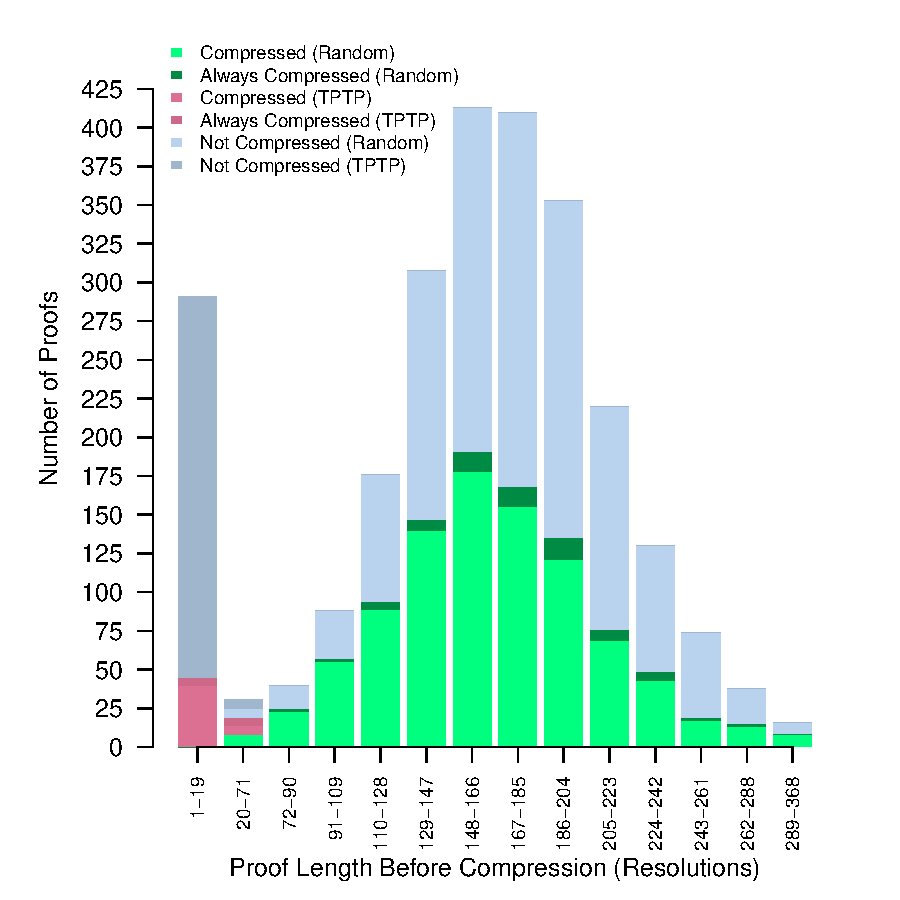
\includegraphics[scale=0.5]{images/combined-all-num_compressed_stacked.pdf} }}
   \subfloat[Compressed length against input length]{{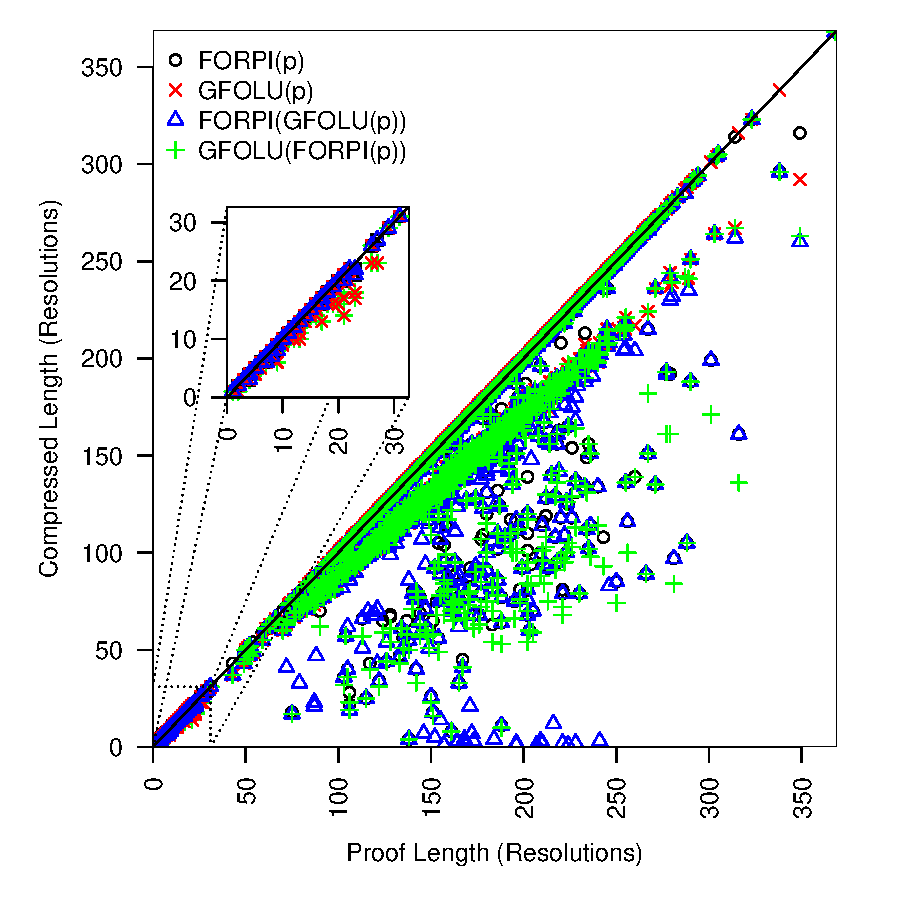
\includegraphics[scale=0.5]{images/combined-all-res-length-vs-compressed-res-length.pdf} }}   
   
  \hspace{-2cm}\subfloat[\FORPI(\GFOLU(p)) vs. \GFOLU(\FORPI(p))]{{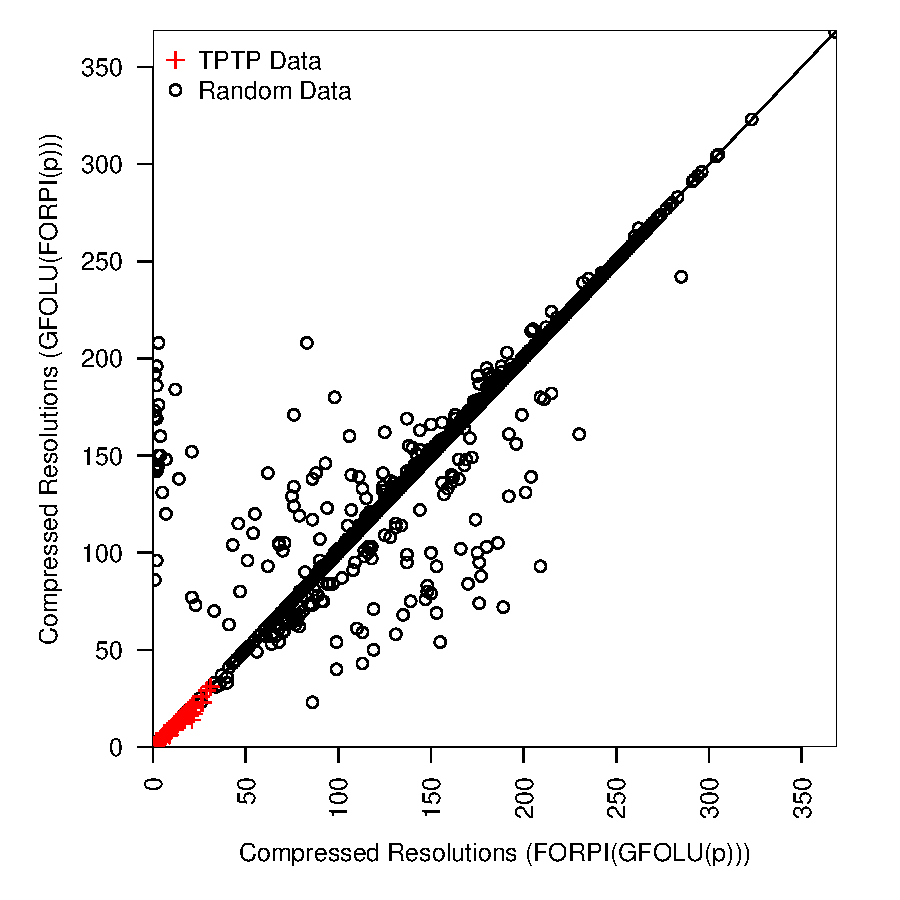
\includegraphics[scale=0.5]{images/combined-alg-res.pdf} }}
  \subfloat[Cumulative proof compression]{{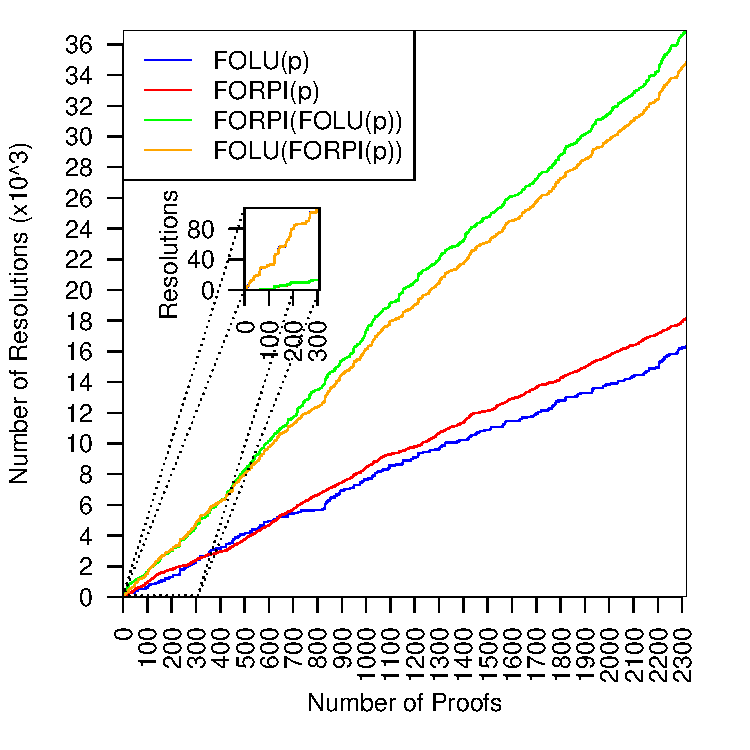
\includegraphics[scale=0.5]{images/combined-all-cumulative-res-nodes-diff.pdf} }}   


 \caption{\GFOLU \& \FORPI Combination Results}
\label{fig:ex}

\end{figure}


